% !TEX root = ../ausarbeitung.tex

\chapter{Anhang}

\section*{Nutzertest}
\label{sec:anhang-test}

\subsection*{Beispieltext}
\begin{figure}[h!]
	Einem reichen Manne, dem wurde seine Frau krank, und als sie fühlte, dass ihr Ende herankam, rief sie ihr einziges Töchterlein zu sich ans Bett und sprach: "Liebes Kind, bleibe fromm und gut, so wird dir der liebe Gott immer beistehen, und ich will vom Himmel auf dich herabblicken, und will um dich sein." Darauf tat sie die Augen zu und verschied. Das Mädchen ging jeden Tag hinaus zu dem Grabe der Mutter und weinte, und blieb fromm und gut. Als der Winter kam, deckte der Schnee ein weißes Tüchlein auf das Grab, und als die Sonne im Frühjahr es wieder herabgezogen hatte, nahm sich der Mann eine andere Frau.
	\caption{Beispieltext \textit{Aschenputtel}}
\end{figure}

\begin{figure}[h]
	\centering
	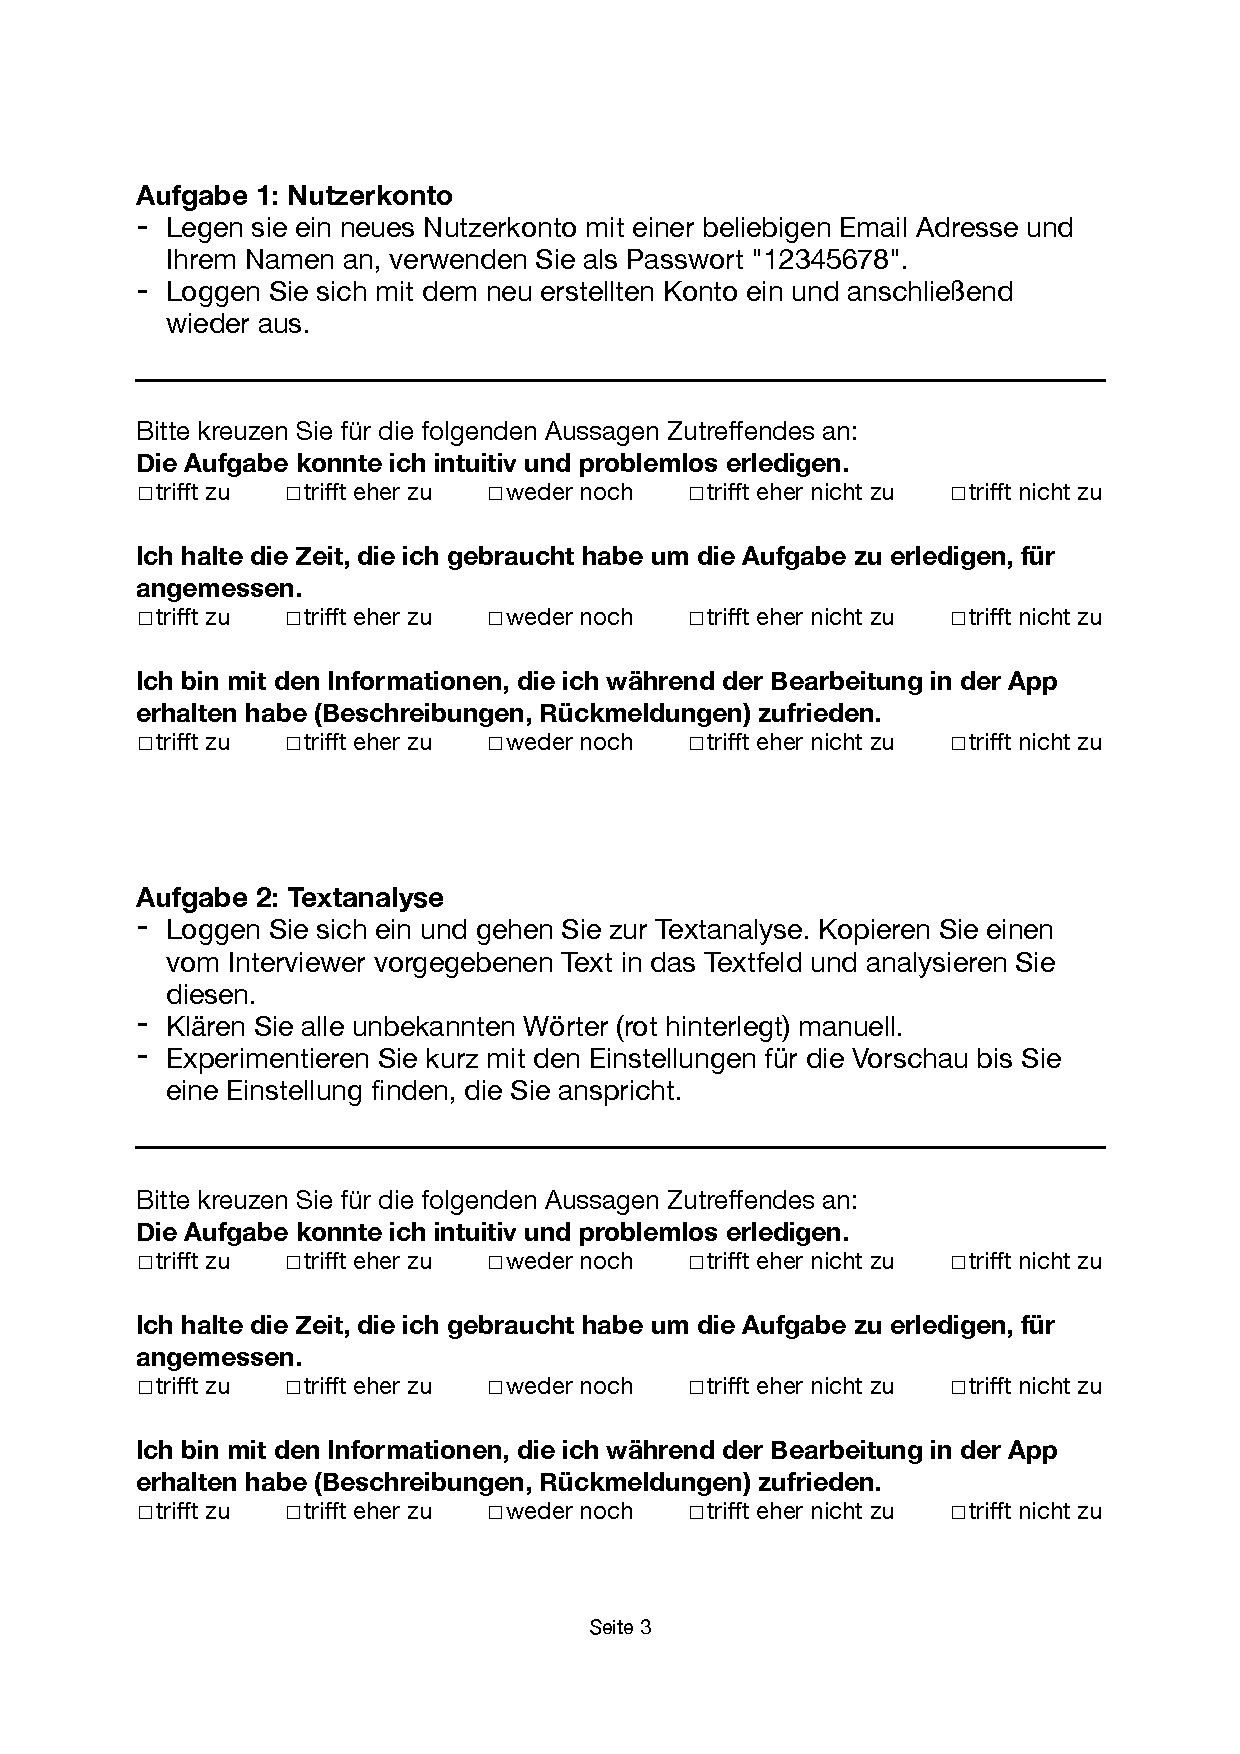
\includegraphics[width=.95\linewidth, frame]{figures/evaluation/test12}
	\caption{Nutzertest: Szenarien 1 und 2}
	\label{fig:evaluation-test12}
\end{figure}
\newpage

\begin{figure}[h]
	\centering
	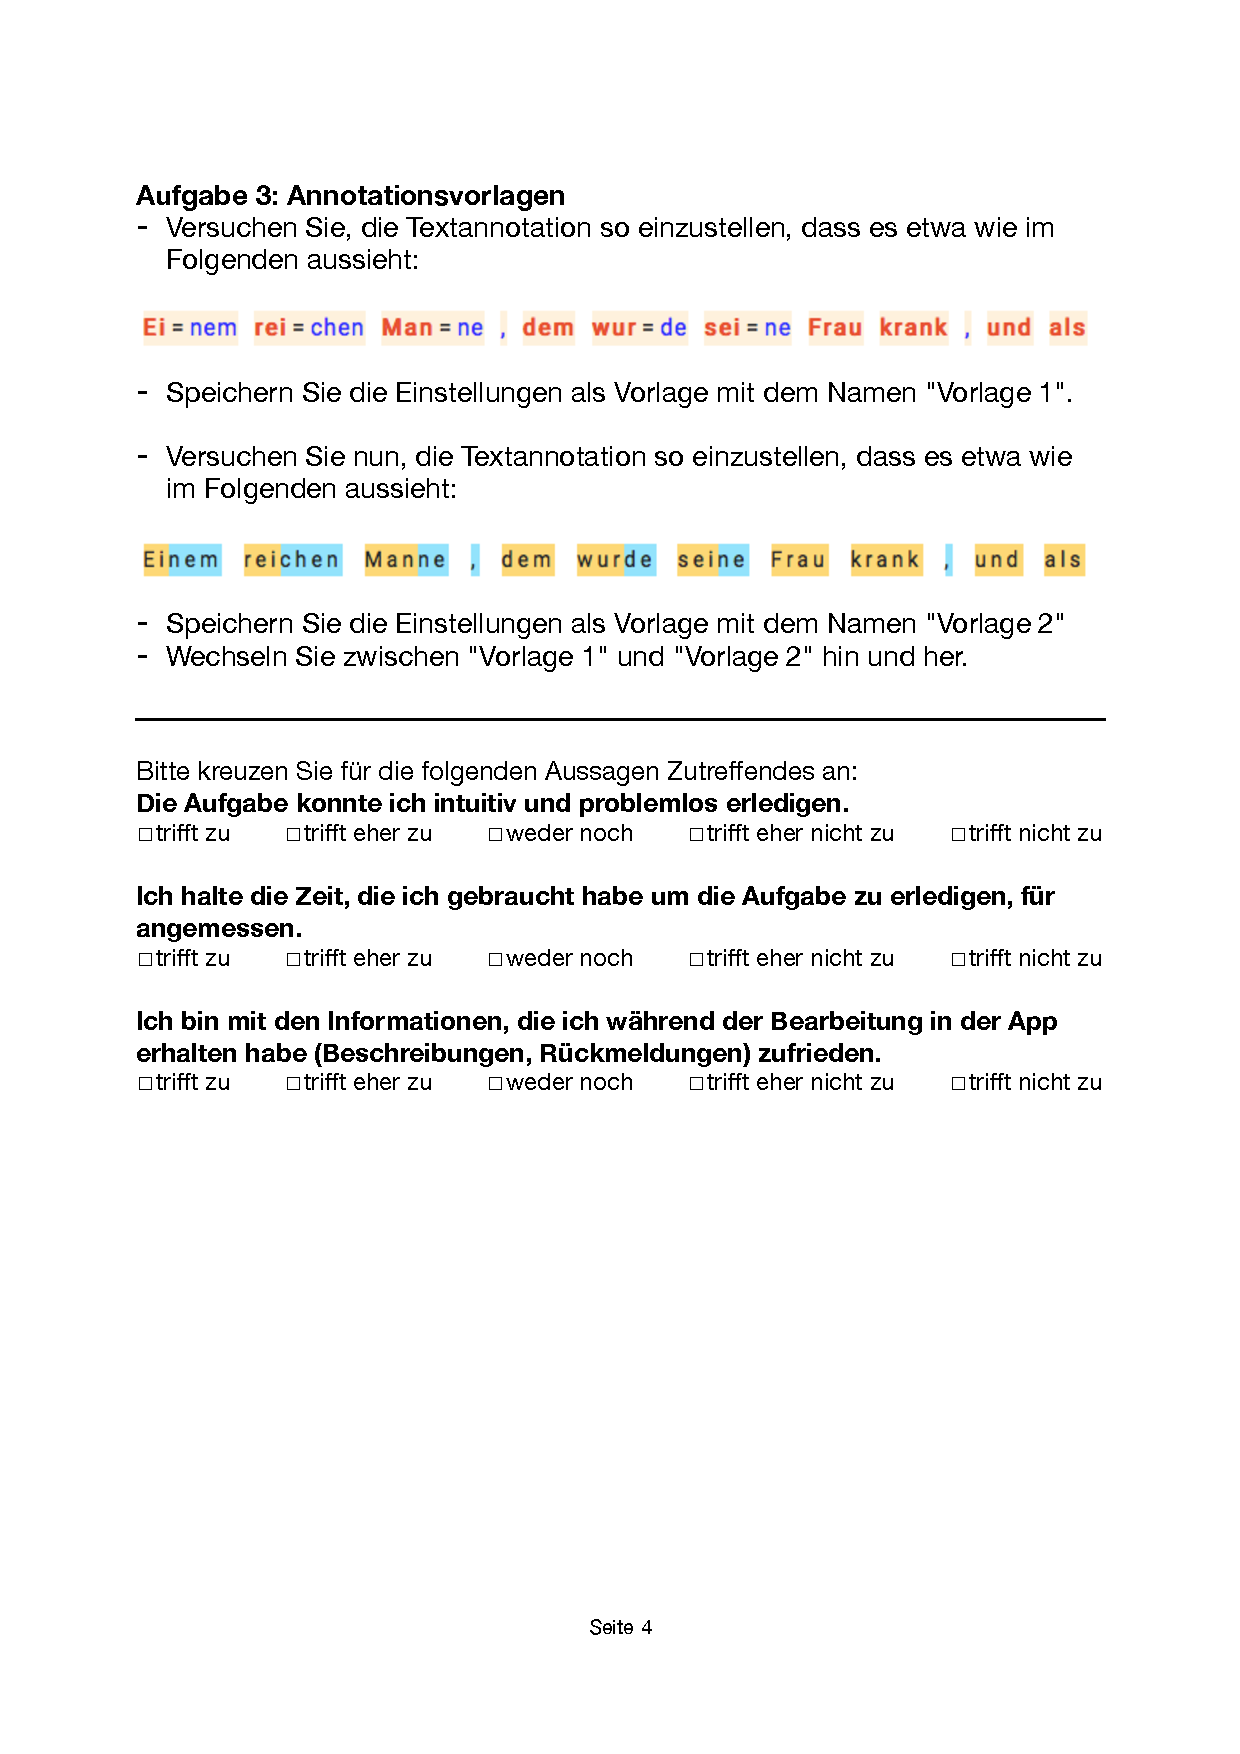
\includegraphics[width=.95\linewidth, frame]{figures/evaluation/test3}
	\caption{Nutzertest: Szenario 3}
	\label{fig:evaluation-test3}
\end{figure}
\newpage

\begin{figure}[h]
	\centering
	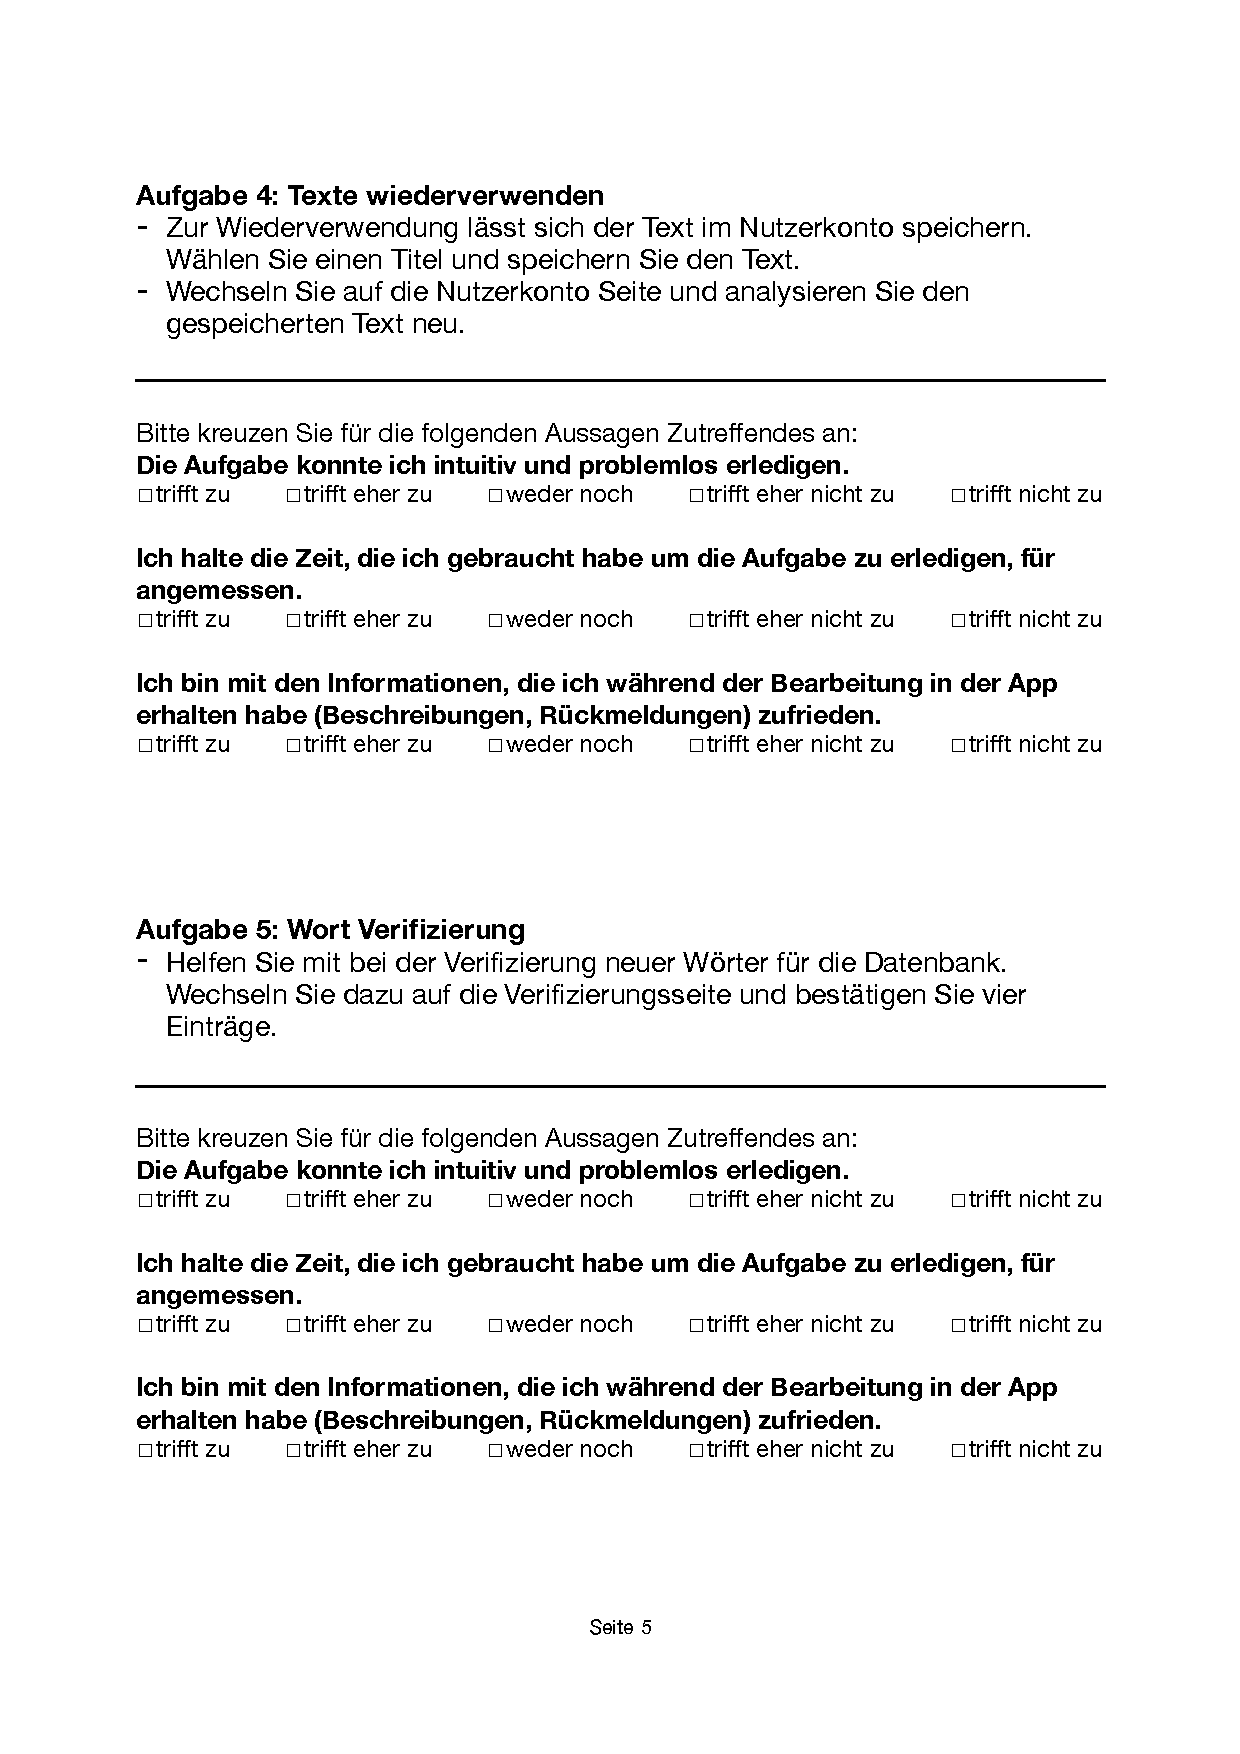
\includegraphics[width=.95\linewidth, frame]{figures/evaluation/test45}
	\caption{Nutzertest: Szenarien 4 und 5}
	\label{fig:evaluation-test45}
\end{figure}
\newpage

\begin{table}[h!]
	\centering
	\begin{tabular}{|p{0.5\textwidth}|p{0.4\textwidth}|}
		\hline
		\textbf{Problem} & \textbf{Lösungsvorschlag}\\
		\hline
		\hline
		Statt ein neues Konto zu erstellen gab die Testperson Email-Adresse und Passwort in das Login Formular ein. & Separate Links in der Navigation für Login/Konto erstellen oder \textit{Neues Konto erstellen} Link auf der Login Seite vor dem Login platzieren.\\
		\hline
		Email und Passwort wurden bei Konto erstellen vergessen, da der Cursor beim Laden der Seite zum Feld \textit{Name} springt. & Cursor ganz nach oben, ins Email Feld setzen.\\
		\hline
		Beim Feld \textit{Name} verwirrte die Beschreibung \textit{Vor- und Nachname werden bei der Verifizierung angezeigt, wenn Sie einen Vorschlag abschicken}. Es war nicht klar, was hier ein \textit{Vorschlag} ist.
		Besser beschreiben, was hier mit Vorschlag gemeint ist (Vorschlag für die Wortsegmentierung bei der Verifizierung). & -\\
		\hline
		Auf der \textit{Home} Seite wurde Login/Konto erstellen nicht gefunden, da es nicht offensichtlich war, das man nach unten scrollen kann. & -\\
		\hline
	\end{tabular}
	\caption{Nutzeranmerkungen zu Szenario 1}
	\label{table:szenario1}
\end{table}
\newpage

\begin{table}[h!]
	\centering
	\begin{tabular}{|p{0.5\textwidth}|p{0.4\textwidth}|}
		\hline
		\textbf{Problem} & \textbf{Lösungsvorschlag}\\
		\hline
		\hline
		Die Einstellungsleiste links geht so weit nach unten, dass beim Ändern der Einstellungen immer wieder hoch und runter gescrollt werden musste. Die Testperson hätte bei den Änderungen lieber den Vorschautext immer im Blick gehabt. & Einstellungen kompakter darstellen, Farbauswahl verkleinern.\\
		\hline
		Das Farbauswahl Fenster war zu umständlich (Fenster musste immer manuell geschlossen werden, Klicken außerhalb funktionierte nicht). & -\\
		\hline
		Die Beschreibungen zu den Einstellungen \textit{Wort Hintergrundfarbe} und \textit{Silbe hervorheben} sind unzureichend und verwirrend. Es wurde nicht selbständig verstanden, was diese tun. & Verständlichere Beschriftung der Optionen (z.B. Schriftfarbe und Hintergrundfarbe). Kurze Erklärung, z.B. Popup bei Hover über ein Info-Symbol.\\
		\hline
		Bei der manuellen Segmentierung lieferten die Vorschläge Wörter ohne Betonung, die es nicht geben sollte. & Nur Vorschläge mit Betonung erlauben.\\
		\hline
		Bei der manuellen Segmentierung wurde der \textit{Speichern} Button nicht gefunden, da nicht klar war, dass nach unten gescrollt werden kann. & -\\
		\hline
		Eine Testperson aus der Expertengruppe vermisste eine schnelle Einstellung, sodass einsilbige Wörter immer in abwechselnden Farben dargestellt werden können. & -\\
		\hline
		Die Satzzeichen waren falsch gesetzt, z.B. müssten Punkte und Kommas immer direkt (ohne Lücke) an das vorherige Wort anschließen. & -\\
		\hline
	\end{tabular}
	\caption{Nutzeranmerkungen zu Szenario 2}
	\label{table:szenario2}
\end{table}
\newpage

\begin{table}[h!]
	\centering
	\begin{tabular}{|p{0.5\textwidth}|p{0.4\textwidth}|}
		\hline
		\textbf{Problem} & \textbf{Lösungsvorschlag}\\
		\hline
		\hline
		Bei der zweiten Einstellung (Hintergrundfarbe pro Silbe und schwarzer Text) wurden die Silbenfarben auf Schwarz gestellt (wegen der Textfarbe). Dass man mit der Option \textit{Silbe hervorheben - Hintergrundfarbe} umstellen kann, ob sich die Silbenfarben auf Schrift- oder Hintergrundfarben beziehen, war nicht klar. & Die Option \textit{Silbe betonen} sollte besser beschrieben werden. Sie sollte an den Anfang der Einstellungen gesetzt werden und ihre Wichtigkeit sollte betont werden (etwa als \textit{Modus} - Schriftfarbe vs. Hintergrundfarbe). Bei den beiden Optionen von \textit{Silbe betonen} sollte jeweils ein hervorgehobenes Beispielwort neben dem Menü verdeutlichen, wie es ungefähr aussehen wird.\\
		\hline
		Statt die Vorlage zu speichern, speicherten Testpersonen den Text mit dem Namen \textit{Vorlage 1}. & -\\
		\hline
		Der Kasten für die Vorlagen befand sich zu weit unten auf der Seite. & \\
		\hline
		Die Meldung \textit{Vorlage angelegt} verschwindet nicht beim Wechseln der Vorlagen, was verwirrend war, weil es sich auf eine vorherige Aktion bezog. & Meldungen sollten sich automatisch schließen, wenn eine neue Interaktion stattfindet.\\
		\hline
		Die Einstellungen wurden als schlecht gruppiert empfunden.  & Farbeinstellungen nebeneinander platzieren (etwa so, wie es im Wort aussieht). Das erleichtert das Verständnis und würde weniger Platz wegnehmen.\\
		\hline
		Eine Testperson aus der Expertengruppe hätte gerne sowohl Schriftfarben als auch Hintergrundfarben individuell angepasst. & -\\
		\hline
		Beim Speichern der Vorlagen war nicht ersichtlich, dass der Vorlagename in einem Textfeld steht und verändert werden kann. & Textfeld besser als solches kennzeichnen.\\
		\hline
	\end{tabular}
	\caption{Nutzeranmerkungen zu Szenario 3}
	\label{table:szenario3}
\end{table}
\newpage

\begin{table}[h!]
	\centering
	\begin{tabular}{|p{0.5\textwidth}|p{0.4\textwidth}|}
		\hline
		\textbf{Problem} & \textbf{Lösungsvorschlag}\\
		\hline
		\hline
		Die Nutzerkonto Seite wurde erst nach längerem Ausprobieren oder nach einem Hinweis gefunden. & Auf der \textit{Home} Seite war der Link immer noch mit \textit{Einloggen oder Konto erstellen} beschriftet. Dies sollte dann \textit{Zum Nutzerkonto} lauten.\\
		\hline
		Es war nicht ersichtlich, dass Texte im Nutzerkonto gespeichert wurden. & -\\
		\hline
		Es war nicht klar, welche \textit{Seite} in der Navigation gerade ausgewählt ist. & In der Navigation sollte die aktuelle Seite hervorgehoben dargestellt werden (z.B. unterstrichen).\\
		\hline
		Die Unterscheidung von Vorlagen und Nutzertexten war nicht klar. Manche Testpersonen dachten, dass die Texte zusammen mit den Vorlagen gespeichert werden. & -\\
		\hline
		Die Beschreibung des Buttons \textit{Verwenden} beim ausgewählten Nutzertext ist nicht einheitlich mit der Textanalyse. & Ändern in \textit{Analysieren}.\\
		\hline
	\end{tabular}
	\caption{Nutzeranmerkungen zu Szenario 4}
	\label{table:szenario4}
\end{table}


\begin{table}[h!]
	\centering
	\begin{tabular}{|p{0.5\textwidth}|p{0.4\textwidth}|}
		\hline
		\textbf{Problem} & \textbf{Lösungsvorschlag}\\
		\hline
		\hline
		Die Beschreibung des Buttons \textit{Abschicken} gefällt nicht. & Ändern in \textit{Bestätigen/Verifizieren}.\\
		\hline
		Bei vielen Vorschlägen ist der Button \textit{Abschicken} zu weit unten. Es war nicht klar, was abgeschickt wird (dass der linke Teil die eigene Segmentierung darstellt). & Der Button sollte zusammen mit der Betonung und Silbentrennung gruppiert sein und direkt darunter stehen.\\
		\hline
		Es wurde als umständlich empfunden, dass immer nur ein Wort auf einmal verifiziert werden kann.
		Eventuell Liste mit Wörtern zum \textit{Abhaken} anzeigen. Vorschläge nur bei bedarf durch Aufklappen anzeigen.
		& -\\
		\hline
		Die manuelle Anpassung der Silbentrennung wurde als umständlich empfunden, da sich der Text nicht verändern lässt (neu schreiben des Textes ist nicht möglich). & Erlauben, das Wort mit Trennstrichen neu zu schreiben, aber kontrollieren, dass der Worttext danach nicht verändert ist.
		Erklärung, dass Text nicht verändert werden kann, sondern nur Trennstriche gesetzt werden können.\\
		\hline
	\end{tabular}
	\caption{Nutzeranmerkungen zu Szenario 5}
	\label{table:szenario5}
\end{table}